
\chapter{引言}
\label{chapter:intro}

\section{研究背景}
当今,人们应该庆幸能够出生在20世纪末,赶上了一个新的计算机技术浪潮,并身处在这个环境中。
有赖于计算机互联网技术,计算机存储和计算技术的快速发展,计算机应用已经深入地影响并改变了人类的生活。

随着计算机技术的广泛应用所带来的互联网信息爆炸,以及大数据处理技术发展已经不再是什么新鲜的话题了。
然而它们给人类带来的机遇和挑战从来不会中断和消逝,因为现代计算机技术的发展的动力正是来源于这种源源不断的冲击。
直面这些问题与挑战,本文以互联网的兴起为大背景,大数据处理技术为基础,展开了对分布式流式主题模型的设计与实现的探索。

\subsection{流式数据}

美国图灵奖得主,诺贝尔经济学奖获得者赫伯特$\cdot$西蒙(Herbert A.Simon, $1916\sim2001$)曾说过:“在信息时代,最稀缺的资源不在是信息本身,而是对信息的处理能力。”

什么是大数据,迄今没有公认的定义。相较于传统的数据,人们将大数据的特征总结为5个V,即体量大(volume)、速度快(velocity)、模态多(variety)、难辨识(veracity)和价值大密度低(value)\cite{cxq2014Survey}。但大数据的主要难点并不在于体量大,真正难以应付的问题来自于其他几种特性。在这种环境下,人们往往遇到的是非结构化,海量实时的文本、视频、语音数据。这些数据常常意味着更大的技术挑战和更复杂的计算,以及更长的计算时间。而在商业应用中,数据处理的时间和质量往往意味着利益。

在许多应用场景中,数据是一个无穷的序列,并且数据的来源各异,格式复杂多样,数据可能带有一些时序,但是有无法保证数据是按照时间顺序排列处理。通常这类数据被称为流式数据。在不同场景下流式数据呈现出不同的特征,但是他们仍然具有鲜明的共性:

(1) 无限性。在流式场景下,数据以元组为单位,以连续的数据流的形式持续地到达计算系统。

(2) 无序性。虽然每个元组会按照某种时间顺序产生,但是,数据并不是严格按照时间次序到达。

(3) 突发性。数据的流速大小、元组特性数量和数据格式无法被提前预知。

(4) 易失性。在流式场景下,累加的数据量非常巨大。通常来说,数据通过简单的计算之后便会被丢弃,而不会别存储。

(5) 实时性。流式数据不仅是实时产生的,而且要求实时的返回计算结果。短时间内无法返回结果的数据,将会很大的影响系统的性能。

许多分布式计算系统都可以实时或接近实时地处理流式数据。常见的处理系统包括Storm, Spark Streaming和Samza。
Storm是一个实时的数据计算系统,使用过程中会先设计好一个用于实时计算的拓扑结构。Storm的数据流单位是元组,每个元组都是一个不可变的数组。
Spark Streaming是核心Spark API的一个扩展。它并不会像Storm那样一次一个地处理数据流。而是在处理之前按照时间间隔预先将其切分为一批次一批次的批处理作业。数据流被抽象为DStream数据结构,每个微处理批次得到一个RDD。
Samza处理数据流是,会分别按次处理每条收到的消息,但是Samza的刘单位既不是元组也不是DStream,而是一条条消息。

\subsection{流式数据场景}
比较典型的流式计算场景包括金融银行业应用、互联网应用和物联网应用\cite{sun2013bdsc}。
在互联网应用场景中,用户通常通过实时发布和分享产生各类数据,这其中最为典型的包括twitter,微博等社交软件的使用。
据统计,互联网上的数据有$75\%$来自于个人用户,主要有文本,图片、音频和视频等数据形式。


随着互联网的快速发展和壮大,网络已经融入到我们生活的方方面面,
用户可以方便的使用互联网进行检索、购物、娱乐、交流等活动。
根据CNNIC发布的《第39次中国互联网发展状况统计报告》显示,截至2016年12月,
我国网民规模达7.31亿,相当于欧洲人口总量,互联网普及率达到$53.2\%$\cite{website:cnnic-39}。

\begin{figure}[htb]\centering
  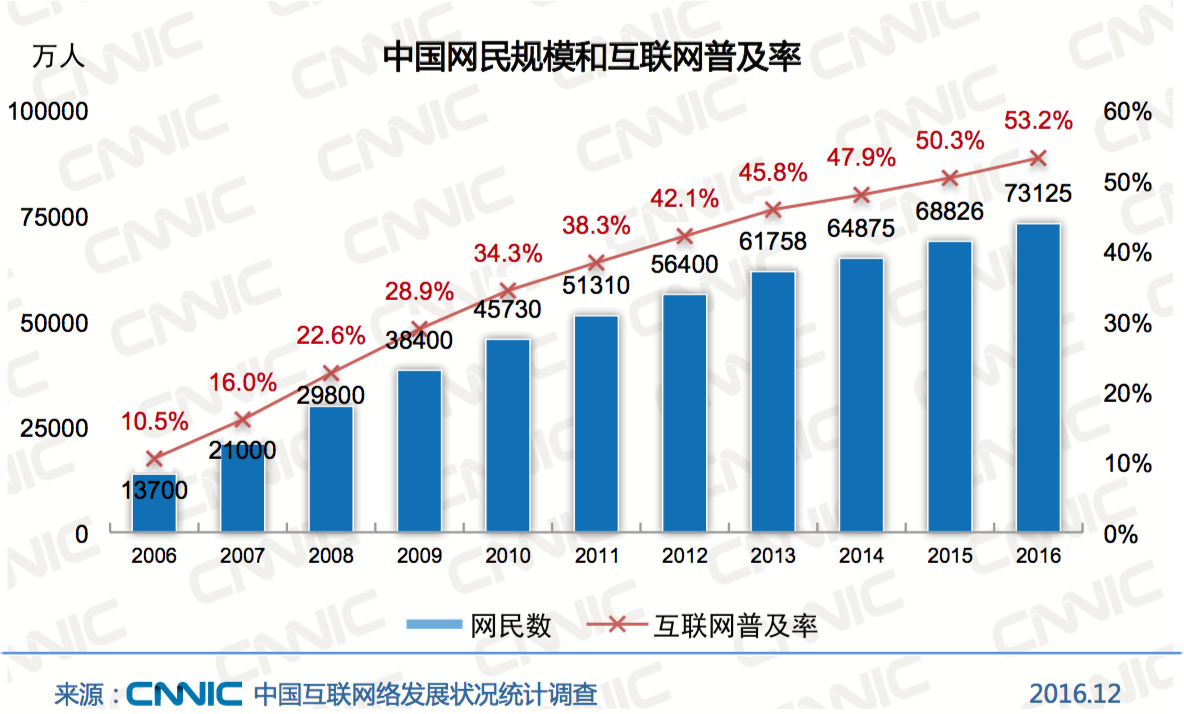
\includegraphics[width=0.7\linewidth]{cnnic-39-netuser}
\caption{中国网民规模和互联网普及率}
\label{fig:cnnic-39-netuser}       % Give a unique label
\end{figure}

社交网络以其快速灵活的方式己经逐渐改变人们交流的方式,用户可以在社交网络上进行沟通、分享、娱乐等活动。
以微博为例,微博是一个拥有庞大的用户基础,月活跃用户数(MAU)达到3亿的社交应用。
相对于传统的社交媒体,微博的时效性更强,影响范围更大,活跃度更高。微博月阅读量超百亿的领域达到了18个。
泛娱乐领域是微博活跃的主力场所;此外,在财经、教育、动漫等领域,微博同样发展迅速,颇受用户关注。
由于微博的流行与普及,微博信息数量呈爆炸式的增长,针对微博数据的处理和应用体现出典型的流式数据处理特征。

\subsection{流式数据与机器学习}
互联网的发展不仅推动了产业革命,同时也促进了机器学习人工智能的发展。人们常说在互联网时代,互联网是基础设施,数据就像原油。
那么机器学习就充当着高效提炼石油的技术。大数据与机器学习人工智能的结合,数据创造价值的关键。
每年Google,Facebook, Microsoft,百度,阿里等等国内外巨头公司都会在这些技术上有巨大的投入。
iResearch预测,2020年,中国人工智能市场将从2015年的12 亿人民币增长至 91 亿人民币。
2015 年,约 14 亿资本(年增长率 $76\%$)流入了中国的人工智能市场。机器学习人工智能俨然已经成为了各大公司的必争之地。

如上面所提及的,社交网络数据带有典型的流式数据特征,类似的场景还有许多。然而在流式数据环境下,传统的批量机器学习方法不再适用。
传统批量机器学习方法在流式数据环境下遇到了如下几个限制:

(1) 有限性

批量机器学习算法为了优化目标函数,会存储有限的训练集。流式数据具有无限性,数据持续的产生和输入,而无法完全存储在内存中。

(2) 迭代性

批量机器学习算法一般需要多轮迭代。在流式场景下,数据具有易失性和实时性,因此对算法的时间效率要求很高。通常数据仅经过简单的计算之后便会被丢弃。
因而,迭代性无法得到保障。

(3) 稳定性

批量机器学习算法都是基于独立同分布假设的。流式环境下,数据的分布可能随时间的推移而变动。因而,独立同分布假设无法得到保证。

(4) 静态性

批量机器学习算法训练得到的模型是静态的。在流式环境下,模型通常需要被实时地更新。使用静态的模型,则模型需要被频繁的替换,从而会造成应用系统的不稳定。

针对这些问题研究者也提出了一些在流式数据上的机器学习算法。
这些算法通常考虑了模型在时间上的延续性,消耗较少的内存,对数据变动具有感知能力。

P.Domingos和G.Hulten\cite{Domingos01catchingup}很好地总结了高效挖掘连续,高速,无尽的数据流学习系统的特性:

(1) 对每个数据样本只需要很少的运算时间

(2) 使用内存大小固定,与处理的样本数据总量无关

(3) 在构建模型的过程中,所有训练数据只会被计算一遍或少数几遍

(4) 随时产生独立于样本顺序的模型

(5) 具有概念迁移能力

\section{研究意义}
主题模型(Topic Model)在机器学习和文本挖掘领域是用来发现一系列文档中潜在语义主题的一种常用统计模型。
作为一个研究方向,主题模型受到了广大计算机科学家的爱戴,许多主题模型的方法被提出并应用于各个领域。
主题模型提供了一种从大规模数据中发现文本潜在语义只是的方法,并且将字词、文档映射到高维的语义空间上。
这种计算对很多语义相关的应用很有帮助,比如信息检索、推荐系统和社交网络等等。
许多公司都有自己的大规模主题模型实现,主要用于广告、推荐和检索等系统中。
不仅如此在生物信息,图像识别以及地理信息等其他学科领域主题模型也有相应的应用。

本文的主要工作是在流式数据环境下实现在线的主题模型。

当谈及流式机器学习的时候,人们往往需要:
(1) 模型具有时效性。比如天气,如果前两天的天气都是晴天40度,那么第三天下雪的可能性就几乎不可能了。
(2) 模型被经常更新。这需要模型对流数据的烟花和结构具有感知。

考虑到流式环境下模型的时效性要求高,模型更新频繁,批量机器学习算法不再适用。
现有的比较具有代表性的对规模主题模型实现包括LightLDA\cite{yuan2015lightlda}和PLDA+\cite{Liu:2011:PPL:1961189.1961198},以及Peacock\cite{Peacock}。
这些算法实现快速高效,扩展性也很好。但是,这些算法实现无一不是为静态数据集设计的。
而在流式数据环境下,算法将面临的是开放无限的数据集,持续增长的词表以及不断演变的数据分布。
显然,现有的算法无法克服上面的问题挑战。

解决这个流式数据上的机器学习的挑战常见的途径是增量学习和在线学习。
区别于批量学习,增量学习和在线学习每次只会适用一小批次的数据(而不是整个数据集),并且数据的信息也可能随着时间的变化而产生变化。
这类方法能够渐进地学习到知识更新演化,并且能修正和加强已有的知识,使得更新后的只是能够适应新的数据,而不必重新对全部数据进行迭代学习。
增量学习和在线学习降低了算法对时间和控件的要求,更适应与流式数据环境。

除此之外,在流式数据环境下主题模型的设计与实现仍然存在一系列挑战:

(1) 流式数据的特点带来的挑战

在流式数据环境下,数据带有实时性和无限性。而经典的主题模型实在静态数据上采用批量学习算法更新模型的,因而无法支持算法的实时性和在线更新。
除此之外,无限的数据意味着动态增长的词表,而词表的大小决定了主题模型的参数个数。根据词汇的幂律分布法则,我们知道随着时间的推移,不断会有新词出现,而绝大多数词汇确实低频词。

(2) 大规模的数据带来的挑战

在社交网络场景下,动辄上亿的数据使得单机机器学习算法无法快速实时地更新模型和作出即使响应。

(3) 主题模型拥有大规模的参数矩阵

主题模型的参数规模,数据词表大小以及主题的维度大小有关。主题模型的参数规模常常超出了一台服务所能存储的容量。不仅如此,在分布式环境下,更多的参数往往意味着更长的网络延迟。

面对如此复杂的算法和应用场景,对主题模型的研究不仅具有现实意义,而且还具有一定的代表性。比如,大规模流式数据上的机器学习模型和大规模参数模型,不仅仅在主题模型这个算法中会出现,同样还会出现在一些其他机器学习算法的应用中。

\section{本文贡献}
如上一节所述,传统的主题模型通常采用批量的机器学习方法训练。
不仅如此,分布式大规模的主题模型通常具有海量的模型参数。
这给模型训练带来了若干个棘手的问题,
a. 海量参数的分布式存储和并行同步;
b. 模型迭代时间随着主题模型规模的增长线性增长;
c. 无法适应持续增长的动态词表。

为了解决分布式流式数据环境下,主题模型实现遇到的挑战。
本文总结并分析了分布式流式数据环境下文本数据的特性,以及主题模型呈现出来的一些特征。
并在分析总结结果的基础之上,提出了分布式流式主题模型设计与实现的具体方案。
总体来说本文的主要贡献在于:

(1) 提出了分布式流式主题模型

大规模的分布式并行主题模型的实现得到了国内外各大公司的重视,在生产环境中得到了广泛的应用,产生了巨大的价值。
尽管这些算法实现具有高效稳定的特性,这些算法实现并不是针对流式数据设计的。
本文针对分布式流式数据提出了两个算法框架,分别是在线流式主题模型和增量流式主题模型。%,实验证明这两个算法是高效,稳定,收敛的。

(2) 采用了高效的Metropolis-Hastings算法

Gibbs采样算法是LDA主题模型参数估计一种主要方法。然而朴素的Gibbs采样算法是一种串行的坐标下降算法,不仅难以实现分布式并行,
而且采样算法的时间与主题维度大小线性相关。这种方法不适用于分布式大规模主题模型。
本文为了实现高效地执行主题模型算法训练过程中的MCMC采样,本文采用的采样算法使用了Alias Table和Metropolis-Hastings算法使得采样复杂度降低到了$O(1)$。
这种采样技术对于分布式流式主题模型的意义重大,不仅提高了采样的效率,同时令采样算法的时间复杂度不再与主题维度大小相关,模型得以训练更大规模的参数。

(3) 提出了稠密和稀疏并存的分布式参数数据结构

在LDA分布式Gibbs采样算法的实现中,参数词汇主题计数$n(w, t)$起到了关键作用。
如何选取和存储参数$n(w, t)$的数据结构,对算法效率的影响巨大。
因为对于超大规模的主题维度,$n(w,t)$中只有少数非零元,也就是说主题模型参数是一个非常稀疏的矩阵。
不仅如此,参数$n(w, t)$是一个与词汇相关的矩阵。在流式环境下,文本数据中不断有新词出现。
这意味着,分布式流式主题模型无法提前预知词汇表的大小,并且直接对主题模型参数进行存取会造成算法存储和时间效率大大降低。
本文提出的稠密和稀疏并存的分布式主题模型参数数据结构,有效地解决了上述两个问题,并大大提升了算法的执行效率。

(4) 优化了分布式流式主题模型的算法实现

本文在实现分布式流式主题模型时,采用了更加紧凑的4字节数据类型(int, float),而非8字节数据类型(long, double),节省了一般的存储空间并提升了网络传输的效率。
除此之外,本文算法还对算法采样顺序进行了优化,使得算法的参数降低了算法的同步代价。在此基础之上实现的参数Pipeline更新充分利用采样过程中的网络带宽。

\section{章节安排}
本文内容一共分为六章,每章内容组织如下:

第一章为引言部分,主要介绍了流式主题模型的相关背景意义和本文的主要贡献。
在本章中,本文首先介绍了流式数据的应用场景和特性,以及流式机器学习的主要难点。
接下来结合主题模型的应用,阐述了主题模型在流式数据上遇到的困难与挑战,
对于这些问题的研究不仅能够拓展主题模型在流式数据上的应用,而且对其他大规模流式机器学习具有参考意义。
最后介绍了本文的主要贡献。

第二章从两个方面介绍了国内外的相关工作以及研究现状。
第一个方面是关于流式学习的研究现状。流式数据挖掘的途径通常有两种一种是基于数据的方案,另外一种是基于任务的方案。
除此之外,本文还介绍了一些相对前沿的流式学习相关技术,主要是在线学习和增量学习技术。
另外一个方面是关于主题模型的研究现状。本文首先介绍了主题模型的发展历史和相关应用背景,之后又介绍了一些主题模型工作的变形。
最后介绍了大规模可扩展主题算法的实现和应用。

第三章介绍了流式主题模型算法设计。
本文首先总结和分析了常见的批量和在线主题模型方案。
本文指出流式主题模型不同于批量主题模型的设计,也不能套用简单的在线主题模型的设计,对于流式主题模型的设计需要考虑到流式数据主要特性。
本文结合了分布式和在线算法的设计思路,提出了两种大规模在线的流式主题模型。

第四章介绍了几种高效采样算法方案。在这一章,本文首先介绍了MCMC算法的应用及其基本理论背景,并介绍了基于MCMC方法的Metropolis-Hastings采样算法。
然后简要介绍了LDA的Gibbs采样算法。之后本文从主题模型的稀疏性出发详细分析和介绍了几种关于LDA的高效采样算法。
这些采样算法对分布式流式主题模型意义重大,它们不仅能够提升算法采样的效率,而且使得模型可以训练更大规模的参数。

第五章介绍了流式主题模型的实现。本章首先介绍了数据并行和模型并行对分布式并行算法的重要意义,以及参数服务器在分布式机器学习算法实现中的重要作用。
然后分析了流式数据环境下,词汇的主要特性和词汇对主题模型参数的影响。在此分析的结果之上,本章提出了稠密和稀疏并存的参数数据结构。
最后在本章提出的参数数据结构的基础之上,本文又介绍了几种优化实现分布式流式主题模型的具体方案。
